
\chapter{Fahrzeuge}


\section{Fahrgestelle}

\begin{table}[htb]%
	\centering
	\caption{Technische Daten}
	\label{tab:chassis:data}
	\begin{tabular}{llr}
		\mytoprule
		Radstand & & \valunit{258}{mm} \\
		Spurweite & & \valunit{155}{mm} \\
		Masse & & \valunit{}{kg} \\
		\mybottomrule
	\end{tabular}
\end{table}


\section{Aktorik}

\subsection{Lenkung}

Die Lenkung ist als Achsschenkel"|lenkung ausgeführt und wird über ein normales Modellbauservo angetrieben.

Das Servo stellt (über einen integrierten P-Regler) einen Sollwinkel, welcher sich über eine Mechanik auf einen Lenkwinkel der Räder überträgt.

Die Kennlinie "`Servowinkel - Lenkwinkel"' ist nicht dokumentiert.

Die Ansteuerung des Servos, \dah die Vorgabe eines Soll-Servowinkels, erfolgt über ein PWM-Signal. Dieses hat eine Frequenz von \valunit{50}{Hz} (wobei diese nicht sonderlich wesentlich ist) mit Impulsbreiten $T_\mrm{puls}$ zwischen \valunit{1}{ms} und \valunit{2}{ms} (die wesentlich sind).

Dabei bedeutet eine Impulsbreite von \valunit{1,5}{ms} die Neutralstellung des Servos, welches (näherungsweise) einer Geradeausstellung der Räder entsprechen sollte. Ein Impulsbreite von \valunit{2}{ms} bedeutet eine maximale Auslenkung des Servos gegen den Uhrzeigersinn (bei Blick auf die Servowelle) was hier einer Lenkbewegung nach rechts entspricht. Eine Impulsbreite von \valunit{1}{ms} entspricht damit einer maximalen Lenkbewegung nach links.

In \figref{fig:Steering:Servo} ist das Ansteuersignal für den Servo dargestellt.

\begin{figure}[htb]%
	\centering
	\begin{tikzpicture}
		\begin{axis}[%
				width=12cm,
				height=3cm,
				scale only axis,
				axis x line = center,
				axis y line = center,
				xlabel={$t$ [ms]},
				ylabel={$u$ [--]},
				xmin=-3, xmax=28,
				%xtick={-500, -250, 0, 250, 500},
				ymin=0, ymax=1.3,
				%ytick={-100, -50, 0, 50, 100},
				legend pos = south east]

		\addplot [
				color=black,
				solid,
				forget plot
				]
			coordinates{
				(-10, 0) (0, 0) (0, 1) (1.5, 1) (1.5, 0) (20, 0) (20,1) (21.5,1) (21.5,0) (40,0)
			};
			
		\draw[black,->] (axis cs:19,0.75) -- (axis cs:20,0.75);
		\draw[black,<-] (axis cs:21.5,0.75) -- node[auto]{$T_\mrm{Puls}$} (axis cs:24,0.75);
			

		%\addplot [
				%color=gray!50,
				%solid,
				%forget plot
				%]
			%coordinates{
				%(-10, 0) (0, 0) (0, 1) (2, 1) (2, 0) (20, 0) (20,1) (22,1) (22,0) (40,0)
			%};

		\end{axis}
	\end{tikzpicture}
	
	\caption{Ansteuerung Servo}%
	\label{fig:Steering:Servo}%
\end{figure}


Das ucboard übernimmt die Ansteuerung des Servos. Dabei wird von außen ein Sollwert zwischen $-1\,000$ und $1\,000$ vorgeben. Dieser Bereich wird auf eine Impulsbreite von 1 bis \valunit{2}{ms} umgerechnet. Die Auf"|lösung der gestellten Impulsbreite beträgt dabei \valunit{1}{\upmu s}. (Damit ist die effektive Auf"|lösung der Stellgröße 2.)

Es ist Folgendes zu beachten:
\begin{itemize}
	\item Die Servos können aufgrund der Lenkmechanik nicht ihren vollen Stellbereich ausnutzen. Dies hört man, wenn ein Sollwert von 1\,000 oder $-1\,000$ vorgegeben wird. Es sollte auf Dauer vermieden werden, Servowinkel zu steuern, die nicht erreichbar sind.
	\item Lenken im Stillstand ist wie bei einem normalen Auto schwerer als in der Fahrt. Es kann je nach Achslast sein, dass das Servo einen gewünschten Lenkwinkel im Stillstand nicht erreicht. 
	\item Die Lenkung besitzt ein gewisses Spiel. (Mit der IMU kann aber die Gierrate bestimmt werden, und damit kann bei bekannter Fahrgeschwindigkeit wiederum auf den Lenkwinkel geschlossen werden. Somit könnte der Lenkwinkel unterlagert geregelt werden.)
\end{itemize}




\subsection{Fahrmotor (Fahrtenregler)}
\label{sec:hw:drivectrl}

Die Fahrzeuge verfügen über Gleichstrommotoren, die über einen Tamiya Fahrtenregler angesteuert werden. Dabei ist bei den Chassis 1 bis 5 ein Tamiya TEU-101BK und bei den Chassis 6 und 7 ein Tamiya TEU-104BK verbaut. (Im Wesentlichen unterscheiden diese sich dadurch, dass bei den TEU-104BK ein Batterieschutz implementiert ist, der jedoch hier deaktiviert ist.)

Die Fahrtenregler werden wie die Lenkung durch ein "`Servo-PWM-Signal"' angesteuert. \Dah eine Pulsbreite von \valunit{1,5}{ms} entspricht "`aus"', kürzere Pulsbreiten einer Vorwärtsfahrt und negative Impulsbreiten einer Rückwärtsfahrt \bzw Bremsen.

Die "`Endanschläge"' (sowie die Neutralstellung) sind dabei kalibrierbar. Hier ist es so kalibiriert, dass die Impulsbreiten \valunit{1}{ms} und \valunit{2}{ms} die Grenzwerte und \valunit{1,5}{ms} die Neutralstellung darstellen.

Da der Fahrtenregler intern gewisse Toleranzzonen berücksichtigt sowie in der Rückwärtsfahrt nur die halbe Stellgröße verwendet, ergibt sich die in \figref{fig:DrvCtrl:charact} gezeigte Kennlinie, wobei $\Delta t_\mrm{Puls}$ die Abweichung der Pulsbreite von \valunit{1,5}{ms} ist,
\begin{align*}
	T_\mrm{Puls} = \valunit{1,5}{ms} + \Delta T_\mrm{Puls}\;.
\end{align*}

\begin{figure}[htb]%
	\centering
	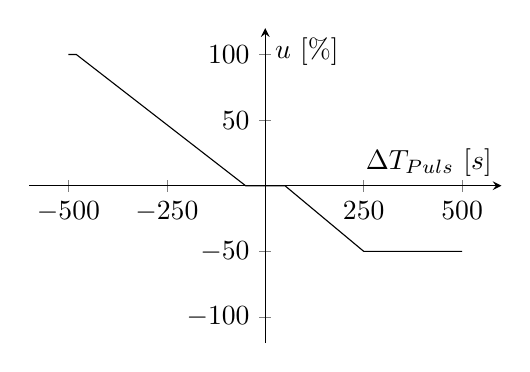
\begin{tikzpicture}
		\begin{axis}[%
				width=6cm,
				height=4cm,
				scale only axis,
				axis x line = center,
				axis y line = center,
				xlabel={$\Delta T_\mrm{Puls}$ $[\mrm{\upmu s}]$},
				ylabel={$u$ [\%]},
				xmin=-600, xmax=600,
				xtick={-500, -250, 0, 250, 500},
				ymin=-120, ymax=120,
				ytick={-100, -50, 0, 50, 100},
				legend pos = south east]

		\addplot [
				color=black,
				solid,
				forget plot
				]
			coordinates{
				(-500,100) (-480,100) (-50,0) (0,0) (50,0) (250,-50) (500,-50)
			};

		\end{axis}
	\end{tikzpicture}
	
	\caption{Kennlinie Fahrtenregler}%
	\label{fig:DrvCtrl:charact}%
\end{figure}

Aufgrund des eigentlichen Einsatzzweckes der Fahrtenregler weisen diese folgendes Verhalten auf:
\begin{itemize}
	\item Negative $\Delta T_\mrm{Puls}$, \dah kleinere Pulsbreiten als die Neutralstellung (außerhalb der Toleranzzone), führen immer zur Vorwärtsfahrt.
	\item Wenn von aus einer Vorwärtsbewegung zu positiven $\Delta T_\mrm{Puls}$ gewechselt wird, dann erfolgt eine Bremsung. Diese wird aber nicht über den Stillstand hinaus ausgeführt, \dah der Fahrtenregler stellt sicher, dass keine Rückwärtsbewegung eintritt.
	\item Um ausgehend von einer Vorwärtsfahrt Rückwärts zu fahren, muss der Fahrtenregler einmal mit positivem $\Delta T_\mrm{Puls}$ angesteuert werden (Bremsen), dann muss der Fahrtenregler mit einer Pulsbreite von \valunit{1,5}{ms} angesteuert werden. Damit ist die Rückwärtsfahrt "`freigeschaltet"'. Wenn jetzt wieder ein positives $\Delta T_\mrm{Puls}$ aufgebracht wird, dann erfolgt eine Rückwärtsfahrt. (Die Einzelschritte dieser Sequenz sind mindestens für \valunit{100}{ms} zu halten. Damit hat sich bisher immer eine sichere Umschaltung ergeben.)
\end{itemize}

Das ucboard bietet zur Ansteuerung zwei Möglichkeiten. Zum einen kann der Fahrtenregler "`direkt"' betrieben werden, \dah man dann den Wert für $\Delta T_\mrm{Puls}$ in Mikrosekunden direkt vorgeben. Die zweite Möglichkeit ist die der "`gemanagten"' Ansteuerung. Hierbei wird dem ucboard mitgeteilt, welche Fahrtrichtung gewählt werden soll und welche Stellgröße dabei verwendet werden soll. Dabei meint ein positiver Wert immer die gewählte Bewegungsrichtung, bei Vorwärtsfahrt bedeutet ein negativer Wert eine Bremsung. Dabei bildet bei Vorwärtsfahrt der Wertebereich von 1 bis 1\,000 den Stellgrößenbereich von 0 bis 100\,\% ab, bei Rückwärtsfahrt wird der Wertebereich von 1 bis 500 auf 0 bis $-50\,\%$ abgebildet. Ein Wert von 0 bedeutet Neutralstellung. Es ergeben sich damit die Kennlinien aus \figref{fig:DrvCtrl:charact_fb}.

\begin{figure}[htb]%
	\centering
	\subfloat[Vorwärts/Bremsen\label{fig:DrvCtrl:charact_f}]{%
		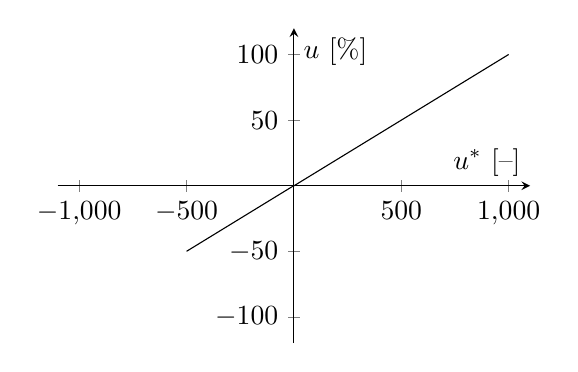
\begin{tikzpicture}
			\begin{axis}[%
					width=6cm,
					height=4cm,
					scale only axis,
					axis x line = center,
					axis y line = center,
					xlabel={$u^*$ [--]},
					ylabel={$u$ [\%]},
					xmin=-1100, xmax=1100,
					xtick={-1000, -500, 0, 500, 1000},
					ymin=-120, ymax=120,
					ytick={-100, -50, 0, 50, 100},
					legend pos = south east]

			\addplot [
					color=black,
					solid,
					forget plot
					]
				coordinates{
					(-500,-50) (-1,0) (0,0) (1,0) (1000,100)
				};

			\end{axis}
		\end{tikzpicture}
	}
	\hspace{2cm}
	\subfloat[Rückwärts\label{fig:DrvCtrl:charact_b}]{%
		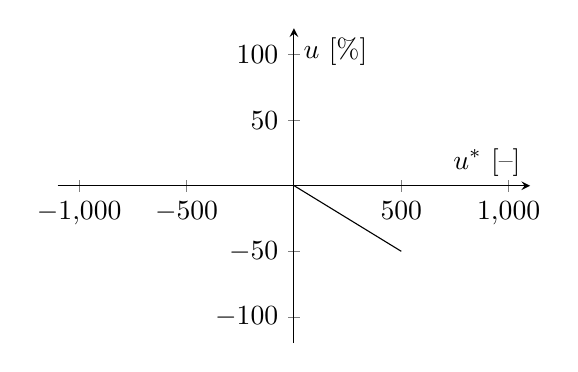
\begin{tikzpicture}
			\begin{axis}[%
					width=6cm,
					height=4cm,
					scale only axis,
					axis x line = center,
					axis y line = center,
					xlabel={$u^*$ [--]},
					ylabel={$u$ [\%]},
					xmin=-1100, xmax=1100,
					xtick={-1000, -500, 0, 500, 1000},
					ymin=-120, ymax=120,
					ytick={-100, -50, 0, 50, 100},
					legend pos = south east]

			\addplot [
					color=black,
					solid,
					forget plot
					]
				coordinates{
					(0,0) (1,0) (500,-50)
				};

			\end{axis}
		\end{tikzpicture}
	}
	\caption{Kennlinien zur "`gemanagten"' Ansteuerung über ucboard}%
	\label{fig:DrvCtrl:charact_fb}%
\end{figure}

Die für die Umschaltung von Vorwärts- auf Rückwärtsfahrt notwendige Bestimmung des Ist-Zustandes des Fahrtenreglers erfolgt dabei über einen Zustandsautomaten, der die Zustandswechsel des Fahrtenreglers nachbildet. Für den normalen Betrieb sollte dies sicher funktionieren. Fehler können nur dann auf"|treten, wenn
\begin{itemize}
	\item sehr schnell zwischen Vor- und Rückwärtsfahrt gewechselt wird (weniger als \valunit{200}{ms} zwischen aufeinanderfolgenden Wechsel) oder
	\item im Direktmodus Werte gestellt werden, die an den Rändern des Toleranzbereichs für die Neutralstellung liegen.
\end{itemize}
Erfolgt eine Vorwärtsfahrt (länger als \valunit{100}{ms}) stimmen die Zustände wieder überein.




Die Fahrtenregler sind hier so angeschlossen, dass \emph{keine} der \valunit{5}{V}-Spannungsversorgungsleitungen angeschlossen ist, sondern die Spannung direkt aus dem Fahrakku nimmt. Die Verbindung zum Fahrakku kann über das ucboard und den drvbatswitch geschaltet werden.



Die notwendige Massenverbindung als Bezug für das PWM-Signal wird über die Verbindung des ucboards mit dem drvbatswitch hergestellt. Dieses muss daher immer angeschlossen sein. (Ansonsten muss (nur!) die Masseleitung des nicht angeschlossenen Spannungsversorgungskabel des Fahrtenreglers an einen Massepin des ucboards angeschlossen werden.) 



\paragraph{Problemlösung}

\begin{itemize}
	\item Schalter des Fahrtenreglers am Chassis auf "`ON"'?
\end{itemize}



\section{Sensorik}

\subsection{Ultraschall}

Es sind drei Ultraschallsensoren des Typs SRF08 verbaut, jeweils einer nach vorne, nach links und nach rechts.

Es wird die Zeit $T_\mrm{echo}$ vom Aussenden des Ultraschallimpulses bis zum Empfang des ersten Echos gemessen.\footnote{Genau genommen werden auch noch möglicherweise auf"|tretende weitere Echos gemessen. Die dazugehörigen Zeiten stellt der Sensor in weiteren Registern zur Verfügung. Aktuell werden diese jedoch nicht ausgelesen. Möglicherweise könnte man mit einer Auswertung dieser Daten Fehlmessungen reduzieren.}

Der gemessene Abstand $d$ entspricht der halben Signallaufstrecke $c \cdot T_\mrm{echo}$, wobei für die Schallgeschwindigkeit $c = \valunit{343,2}{m/s}$ angenommmen wird. Es ergibt sich damit
\begin{align*}
	d = \frac{1}{2} \cdot c \cdot T_\mrm{echo} = \valunit{171,6}{\frac{m}{s}} \cdot T_\mrm{echo}\;.
\end{align*}


Der Sensor gibt die Zeiten $T_\mrm{echo}$ in Mikrosekunden zurück, wobei die Auf"|lösung \valunit{4}{\upmu s} ist. Damit ergibt sich eine Distanzauflösung von \ca \valunit{0,7}{mm}. Die Messwerte werden vom ucboard in \valunit{0,1}{mm} zurückgegeben.


\paragraph{Optionen: Messbereich und Verstärkung}

Siehe Datenblatt des Sensors.


\subsection{Hall-Sensor}

Mit dem Hall-Sensor (Typ HAL 503) kann die Drehzahl des hinteren linken Rades gemessen werden. Dazu sind auf der Felge des Rades über den Umfang acht Magnete verteilt, die von der Polarität her immer wechselweise angeordnet sind.

Der genannte Sensor besitzt zwei stabile Zustände. Wird ein positiver magnetischer Pol in die Nähe gebracht, so wechselt er in den Zustand 1, bei einem negativen magnetischen Pol in den Zustand 0. Liegt kein Feld vor, dann wird der alte Zustand gehalten. 

Somit kann durch Messen der Zeit zwischen zwei Zustandswechseln die Zeitdauer für eine achtel Umdrehung bestimmt werden. 

Auf dem ucboard wird die Zeit zwischen den Impulsen auf eine Mikrosekunde genau bestimmt. Die Ausgabe der Messwerte erfolgt dann in \valunit{0,1}{ms}. Daneben wird auch die Summe dieser Zeiten über acht Zustandswechsel, also einer Radumdrehung, bestimmt und in einer Genauigkeit von \valunit{1}{ms} ausgegeben. Zuletzt erfolgt auch die Ausgabe der Anzahl an gezählten Zustandswechseln in Modulo 256, wenn extern selber mitgezählt werden soll. (Letzteres erlaubt auch die Überprüfung, ob ggf. Messdaten verloren gegangen sind.)

Im Gegensatz zu einem "`klassischen"' Encoder kann die Drehrichtung nicht festgestellt werden!

\begin{itemize}
	\item Der Abstand zwischen Rad und Aufbau darf nicht zu groß sein. Ist das Fahrzeug beispielsweise aufgebockt, so werden in der Regel keine Impulse mehr gezählt.\footnote{Vom Hersteller gibt es noch einen Hall-Sensor aus der gleichen Baureihe (HAL 502), der jedoch etwas empfindlicher (die notwendige Flussdichte beträgt \ca ein Drittel im Vergleich zum HAL 503) ist. Sollten häufig Probleme mit übersprungenen Impulsen auf"|treten, wäre dies eine mögliche Lösung.}
\end{itemize}


\subsection{IMU}

Auf der hinteren rechten Ecke des ucboards befindet sich ein Beschleunigungs- und Drehratensensor (IMU -- Inertial Measurement Unit) des Typs MPU-9250A.

Die $x$-Achse zeigt nach vorne, die $y$-Achse nach links und die $z$-Achse nach oben.

Der Sensor gibt die Messwerte als \texttt{int16\_t}-Werte aus. Die Umrechnung eines Sensorwertes \texttt{val} in eine physikalische Einheit hängt von dem gewählten Messbereich ab. Für Beschleunigungswerte gilt
\begin{align}
	a(\mathtt{val})
		=
			\begin{cases}
				\frac{\mathtt{val}}{16\,384} g & \tn{wenn Messbereich } \pm 2\,g \\
				\frac{\mathtt{val}}{8\,192} g & \tn{wenn Messbereich } \pm 4\,g \\
				\frac{\mathtt{val}}{4\,096} g & \tn{wenn Messbereich } \pm 8\,g \\
				\frac{\mathtt{val}}{2\,048} g & \tn{wenn Messbereich } \pm 16\,g 
			\end{cases}
	\label{eq:hw:IMU:ACCScale}
\end{align}
und für Drehratenwerte gilt
\begin{align}
	\omega(\mathtt{val})
		=
			\begin{cases}
				\frac{\mathtt{val}}{131} \mrm{\degree / s} & \tn{wenn Messbereich } \pm \valunit{250}{\degree / s} \\
				\frac{\mathtt{val}}{65,5} \mrm{\degree / s} & \tn{wenn Messbereich } \pm \valunit{500}{\degree / s} \\
				\frac{\mathtt{val}}{32,8} \mrm{\degree / s} & \tn{wenn Messbereich } \pm \valunit{1000}{\degree / s} \\
				\frac{\mathtt{val}}{16,4} \mrm{\degree / s} & \tn{wenn Messbereich } \pm \valunit{2000}{\degree / s}\;.
			\end{cases}
	\label{eq:hw:IMU:GYROScale}
\end{align}

Standardmäßig sind die Messbereiche $\pm 4\,g$ und $\pm \valunit{500}{\degree / s}$ eingestellt. Diese können jedoch über entsprechende Befehle geändert werden.


\paragraph{Filterung}

Die IMU verfügt über digitale Filter, die vor der sensorinternen Unterabtastung angewendet werden. (Der genaue Aufbau der Filter ist nicht dokumentiert. Die Angabe über Bandbreite und Verzögerung ("`delay"') lassen aber darauf schließen, dass es sich im Wesentlichen um eine Mittelwertbildung handelt.) Die möglichen Einstellungen, die über die ucboard-Befehle vorgenommen werden können, sind in \tabref{tab:hw:imufilters} aufgeführt. Diese Werte sind den Einträgen in der "`Register Map"'-Dokumentation des MPU-9250 entnommen. 

\textbf{Hinweis:} Es ist zu beachten, dass die Abtastung (das Abfragen des Sensorwerte) seitens des ucboard unabhängig von der in \tabref{tab:hw:imufilters} \bzw im Sensordatenblatt genannten Abtastszeit immer mit \valunit{1}{kHz} erfolgt! Auch deshalb sollten die in \tabref{tab:hw:imufilters} grau geschriebenen Einstellungen nur zu Informationszwecken verwendet und nicht für den Normalbetrieb vorgesehen werden.

Die Standardeinstellung der Filter ist jeweils \verb|0|.

\begin{table}%
	\centering
	\caption{Filtereinstellungen IMU}
	\label{tab:hw:imufilters}
	\subfloat[Gyroskop \label{tab:hw:imufilters:gyro}]
	{%
		\begin{tabular}{cccc}
			\mytoprule
			\texttt{GFILT} & Bandbreite [Hz] & Verzögerung [ms] &  Interne Sensor- \\
			& & & abtastzeit [kHz] \\
			\mymidrule
			\color[rgb]{0.5,0.5,0.5}{\texttt{-2}} & \color[rgb]{0.5,0.5,0.5}{8\,800}   & \color[rgb]{0.5,0.5,0.5}{0,064} & \color[rgb]{0.5,0.5,0.5}{32}\\
			\color[rgb]{0.5,0.5,0.5}{\texttt{-1}} & \color[rgb]{0.5,0.5,0.5}{3\,600}   & \color[rgb]{0.5,0.5,0.5}{0,11} & \color[rgb]{0.5,0.5,0.5}{32} \\
			\texttt{0} & 250 & 0,97 & 8 \\
			\texttt{1} & 184 & 2,9 & 1 \\
			\texttt{2} & 92   & 3,9 & 1 \\
			\texttt{3} & 41  & 5,9 & 1 \\
			\texttt{4} & 20  & 9,9 & 1 \\
			\texttt{5} & 10  & 17,85 & 1 \\
			\texttt{6} & 5  & 33,38 & 1 \\
			\color[rgb]{0.5,0.5,0.5}{\texttt{7}} & \color[rgb]{0.5,0.5,0.5}{3\,600}  & \color[rgb]{0.5,0.5,0.5}{0,17} & \color[rgb]{0.5,0.5,0.5}{8} \\
			\mybottomrule
		\end{tabular}%
		}
	\\[10mm]
	\subfloat[Beschleunigungssensor \label{tab:hw:imufilters:acc}]
	{%
		\begin{tabular}{cccc}
			\mytoprule
			\texttt{AFILT} & Bandbreite [Hz] & Verzögerung [ms] &  Interne Sensor- \\
			& & & abtastzeit [kHz] \\
			\mymidrule
			\color[rgb]{0.5,0.5,0.5}{\texttt{-1}} & \color[rgb]{0.5,0.5,0.5}{1\,046} & \color[rgb]{0.5,0.5,0.5}{0,503} & \color[rgb]{0.5,0.5,0.5}{4} \\
			\texttt{0} & 218,1 & 1,88 & 1 \\
			\texttt{1} & 218,1 & 1,88 & 1 \\
			\texttt{2} & 99    & 2,88 & 1 \\
			\texttt{3} & 44,8  & 4,88 & 1 \\
			\texttt{4} & 21,2  & 8,87 & 1 \\
			\texttt{5} & 10,2  & 16,83 & 1 \\
			\texttt{6} & 5,05  & 32,48 & 1 \\
			\texttt{7} & 420   & 1,38 & 1 \\
			\mybottomrule
			\multicolumn{3}{p{8cm}}{\color[rgb]{1,0,0} \tiny Die Einstellungen \texttt{0} und \texttt{1} sind in der Dokumentation tatsächlich identisch angegeben. Das könnte man mal überprüfen.}
		\end{tabular}
		}
\end{table}



\subsection{Magnetometer}

Das Magnetometer vom Typ AK8963C ist im Gehäuse der IMU integriert. (Prinzipiell empfiehlt es sich, direkt das Datenblatt des AK8963 zu verwenden, und nicht in die entsprechenden Passagen des Datenblattes der IMU zu schauen.)

Die Achsenanordnung des Magnetometers unterscheidet sich von der der IMU \bzw damit auch der Achsenanordnung des Fahrzeugs. So zeigt die $x$-Achse zeigt nach links, die $y$-Achse nach vorne und die $z$-Achse nach unten. \textbf{\emph{Alle} ausgegebenen Werte werden jedoch in Fahrzeug- oder IMU-Koordinaten angegeben!}

Es liegt \ca alle \valunit{10}{ms} neue Messwerte vor. (Ungefähr, da die Taktrate des Mikrocontrollers und die des Sensors leicht abweichen können.)


\paragraph{Korrektur der Sensorempfindlichkeit}

Im Magnetometer ist intern für jede Achse ein Korrekturwert für die Sensitivität gespeichert (\texttt{ASAX}, \texttt{ASAY} und \texttt{ASAZ}). Dieser wird beim Starten ausgelesen und zur Korrektur der Messwerte verwendet. Diese Korrektur kann auch abgeschaltet werden (\verb|!MAG OPT ~USEASA=0|).

Der korrigierte Wert $H'_{\{\mrm{x,y,z}\}}$ ergibt sich aus dem Sensorwert $H_{\{\mrm{x,y,z}\}}$ und dem jeweiligen Korrekturfaktor \texttt{ASA}\{\texttt{X},\texttt{Y},\texttt{Z}\} über
\begin{align*}
	H'_{\{\mrm{x,y,z}\}} = H_{\{\mrm{x,y,z}\}} \cdot \left( \frac{(\mathtt{ASA}\{\mathtt{X},\mathtt{Y},\mathtt{Z}\} - 128) \cdot 0,5}{128} + 1 \right)\;.
\end{align*}


\paragraph{Kalibrierung des eingebauten Sensors}

Eine weitere Kalibrierung des Magnetometers ist für die Zukunft vorgesehen. Aktuell muss dies aber, wenn gewünscht \bzw notwendig, selber auf dem PC realisiert werden.


\paragraph{Berechnung des Kurswinkels}

Unter der Annahme, dass das Fahrzeug eben steht, kann aus dem Messwert der magnetischen Feldstärke in $x$- und $y$-Richtung der im(!) Uhrzeigersinn gezählte Kurswinkel $\psi_\mrm{h}$ über
\begin{align*}
	\psi_\mrm{h} = \mrm{atan2}(\mathtt{MY},\ \mathtt{MX})
\end{align*}
in Radiant bestimmt werden. Die Funktion atan2 gibt einen Wert zwischen $-\uppi$ und $\uppi$ zurück. Einen typischen "`Kompasswert"' in Grad erhält man daher nach dem Pseudocode
\begin{verbatimtab}[4]
	heading = atan2(MY, MX) * 180 / pi
	
	if heading < 0
		heading = 360 + heading
	end
\end{verbatimtab}



\section{Taster und LEDs}

Auf dem Board sind drei Taster (A, B und C) und zwei LEDs (A und B) vorhanden, die über die serielle Schnittstelle abgefragt \bzw gesetzt werden können. Für die LEDs SYS, DRVBAT und 12V ON ist keine externe Steuerung vorgesehen.


\paragraph{Abfrage Taster}

Die Abfrage der Tasterzustände erfolgt über die DAQ-Kanäle \verb|PBA|, \verb|PBB| und \verb|PBC|. Jeder dieser Kanäle gibt einen Zählerwert der Tasterbetätigungen zurück. Dieser Zähler wird für jedes Herunterdrücken und jedes Loslassen des Tasters inkrementiert. Ein betätigter Taster ist dabei durch eine gerade, und ein unbetätigter Taster durch eine ungerade Zahl repräsentiert. Auf diese Weise lassen sich auch sehr kurze Betätigungen erfassen, ohne dass die Abtastzeit des Kanals sehr klein eingestellt werden muss. Die Zähler sind Modulo 256.

\paragraph{LEDs}

Die LEDs können über einen entsprechenden Befehl ein- und ausgeschaltet werden. Auch können Blinksequenzen vorgegeben werden. Siehe dazu die Befehlsbeschreibung des Befehls \verb|LED|.

